\section{Codierung}
% Was ist eine Codierung
Unter der Codierung eines Individuums versteht man eine Informationskette, welche die relevanten Erbinformationen enthält.
% Codierung in der Natur
Die Gene eines Menschen können so als dessen Codierung angesehen werden.
% Codierung bei den Evolutionsstrategien
Bei den Evolutionsstrategien wurde auf eine komplizierte Codierung verzichtet und dafür eine sehr kurze Codierungsform eingesetzt \cite[S.~147]{schoeneburg}. Die relevanten Erbinformationen von Individuen werden durch Vektoren reeller Zahlen dargestellt \cite[S.~147]{schoeneburg}. Diese Vektoren werden Chromosome genannt. Jedes Individuum besitzt ein solches Chromosom und bildet somit einen validen Lösungsvorschlag des vorliegenden Optimierungsproblems.
Eine Kollektion von Individuen bildet eine Population zur Kapselung des Entwicklungsprozesses. Diese Codierungsweise wird in der Grafik \ref{fig:codierung} dargestellt. Die Individuen sind als Männchen dargestellt. Darüber hinaus ist ein Chromosomausschnitt zu sehen, welcher einen Teil der Parameterausprägungen veranschaulicht.\\
Die Wahl für diese Codierungsvariante lässt sich darauf zurückführen, dass die Evolutionsstrategien zu Beginn für ingenieurstechnische Optimierungen verwendet wurden \cite[S.~147]{schoeneburg}.
In diesem Aufgabenfeld werden auch optimale Systemparameter gesucht. Diese lassen sich sehr gut als Vektoren reeller Zahlen abbilden.\\
Der durch die Evolutionsstrategien gewählte Codierungsansatz wird als phänotypisch orientiert bezeichnet \cite[S.~148]{schoeneburg}. Das bedeutet, dass im Gegensatz zu einer genotypischen Orientierung, die Eigenschaft des Individuums betrachtet wird, die sich aus den Chromosomen ergeben, und nicht die Chromosome selbst.
Die Eigenschaft des Individuums kann durch Qualitätsfunktionen berechnet und somit bewertet werden.

\begin{figure}[!htb]
	\centering
	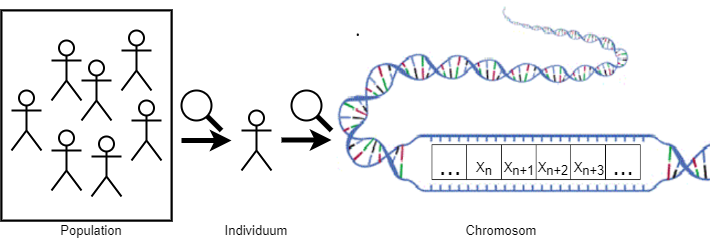
\includegraphics[width=1.\textwidth]{img/codierung/codierung.png}
	\caption{Grafische Darstellung einer Population, von Individuen und eines Chromosoms}
\label{fig:codierung}
\end{figure}
